\documentclass[a4paper,fleqn]{cas-dc}
\usepackage[numbers]{natbib}
\usepackage{siunitx}

\shorttitle{Robust PID tuning under actuator saturation in exothermic CSTRs}
\shortauthors{G.M. de Andrade and E.R. Edwards}

\begin{document}
\let\WriteBookmarks\relax
\def\floatpagepagefraction{1}
\def\textpagefraction{.001}

\title [mode = title]{Robust PID Tuning under Actuator Saturation in Nonlinear Exothermic CSTRs: Performance, Anti-Windup and Sensitivity Trade-offs}

\author[1]{Gabriel Marques de Andrade}
\cormark[1]
\ead{gmandrade.egm@uesc.br}
\credit{Conceptualization, Methodology, Software, Investigation, Writing -- original draft}

\author[1]{Elilton Rodrigues Edwards}
\ead{eredwards@uesc.br}
\credit{Supervision, Methodology, Writing -- review \& editing}

\affiliation[1]{organization={Department of Exact and Technological Sciences (DCET), State University of Santa Cruz (UESC)},
    addressline={Rodovia Jorge Amado, km 16},
    city={Ilh\'eus},
    postcode={45662-900},
    state={Bahia},
    country={Brazil}}

\cortext[1]{Corresponding author}

\begin{abstract}
Benchmarks of PID tuning rules on exothermic reactors often conclude that empirical rules fail, without separating the rule from the actuator model and the anti-windup logic. This paper evaluates eight PID tunings (Ziegler--Nichols, Cohen--Coon, Tyreus--Luyben, AMIGO and its two-degree-of-freedom variant, Skogestad SIMC, and multi-start ITAE optimization subject to a sensitivity peak $M_s \le 1.6$ on the identified dead-time loop, with its two-degree-of-freedom variant) on a three-state nonlinear CSTR whose cooling valve is limited in amplitude and in slew rate. A directional clamping rule that freezes the integrator whenever amplitude or rate saturation cuts the command, with the sign of the reverse-acting loop built in, keeps every tuning stable. A textbook amplitude-only rule lets Ziegler--Nichols and Cohen--Coon wind up during the rate-limited ramp, raising the integral absolute error of a $-2$~K step from $0.940$ to $104.123$~K$\cdot$min. With correct anti-windup, robustness rather than stability separates the rules: high-gain loops inject the most sensor noise into the reactor across $1200$ Monte Carlo runs, and Sobol indices show that the tracking-error variance of every tuning is governed by feed concentration and heat-transfer capacity, while kinetics and sensor delay drive the valve activity of low-margin loops. The constrained optimal PID gives the fastest robust servo response, and setpoint weighting removes overshoot without altering regulation.
\end{abstract}

\begin{highlights}
\item Rate-aware directional clamping keeps all eight PID tunings stable on the CSTR
\item Amplitude-only anti-windup makes the empirical rules lose temperature control
\item High-gain tunings inject the most sensor noise into the reactor temperature
\item Sobol: feed and heat transfer govern error; kinetics and delay drive valve wear
\end{highlights}


\begin{keywords}
Exothermic CSTR \sep Robust PID tuning \sep Anti-windup \sep Rate saturation \sep Pareto trade-off \sep Sobol indices
\end{keywords}

\maketitle

\section{Introduction}\label{sec:intro}
PID controllers still regulate the large majority of loops in the chemical process industries \cite{astrom2006pid, seborg2010process}, and the temperature loop of an exothermic continuous stirred tank reactor (CSTR) is one of the most demanding among them. Arrhenius kinetics couple reactor temperature and reaction rate through an exponential positive feedback, which produces steady-state multiplicity, parametric sensitivity and open-loop unstable regimes \cite{uppal1974dynamic, aris1958analysis, bequette2003process}. The cooling valve that closes the loop is bounded in stroke and in travel speed, and when an aggressive controller drives it into saturation the loop is effectively opened and the integrator winds up \cite{hippe2006windup, tarbouriech2009antiwindup}.

The tuning rules most often used as references for this loop are the reaction-curve rules of Ziegler and Nichols (1942) \cite{ziegler1942optimum} and Cohen and Coon (1953) \cite{cohen1953theoretical}, derived for linear, unconstrained processes \cite{odwyer2009handbook, shinskey1996process}. Their failure on exothermic reactors is a recurring finding \cite{visioli2006practical, luyben2007chemical}, and it is frequently used to motivate model-based, nonlinear or learning-based alternatives. Two aspects of such comparisons are rarely examined. First, the empirical rules are a strawman: modern robust rules such as Tyreus--Luyben \cite{tyreus1992tuning}, AMIGO \cite{astrom2004revisiting}, Skogestad's SIMC \cite{skogestad2003simple, grimholt2018optimal} and $M_s$-constrained optimization \cite{garpinger2014performance, padula2012optimal} are the relevant linear baselines. Second, the verdict on a tuning rule depends on how the actuator and the anti-windup logic are modelled. A clamping rule that checks only the amplitude limits, and that ignores the sign of a reverse-acting loop, keeps integrating while a rate-limited valve ramps towards its target; the resulting windup is then attributed to the tuning rule rather than to the implementation.

This paper separates these effects on a three-state CSTR model with an explicit jacket balance and a cooling valve limited to $[0, 300]$~L/min and $80$~L/min$^2$. Eight PID tunings are compared under one protocol, with error metrics evaluated on the true reactor temperature. The contributions are:
\begin{enumerate}
    \item A directional clamping anti-windup rule that freezes the integrator whenever the previous command was cut by the amplitude \emph{or} the slew-rate limit and the integral increment pushes further into saturation, with the sign of the reverse-acting loop built in. An ablation against the textbook amplitude-only rule shows that the implementation, not the tuning rule, decides whether the empirical rules lose the reactor.
    \item A benchmark of eight tunings---Ziegler--Nichols, Cohen--Coon, Tyreus--Luyben, AMIGO and its two-degree-of-freedom (2-DOF) variant, SIMC, and multi-start ITAE optimization with $M_s \le 1.6$ evaluated on the identified dead-time loop, with its 2-DOF variant---covering servo tracking, unmeasured load disturbances and the robustness margins of the design model and of the exact linearized plant.
    \item A continuous map of the trade-off between tracking error and valve travel obtained by sweeping the SIMC closed-loop time constant and by scalarized optimization \cite{alcantara2013simple, reynoso2021multiobjective}.
    \item A stochastic and global sensitivity analysis: $1200$ Monte Carlo runs under thermocouple noise and Sobol' indices \cite{sobol2001global, saltelli2010variance} of the tracking error and valve travel under simultaneous uncertainty in kinetics, heat transfer, feed concentration and sensor dead time.
\end{enumerate}
Section~\ref{sec:model} presents the plant and the actuator limits, Section~\ref{sec:pid} the controller structure, the anti-windup rule and the tuning rules, Section~\ref{sec:results} the results and Section~\ref{sec:conclusion} the conclusions.


\section{Plant model and actuator limits}\label{sec:model}
\subsection{Nonlinear CSTR model}
An irreversible, exothermic, liquid-phase reaction $A \rightarrow B$ takes place in a CSTR cooled by a jacket \cite{luyben2007chemical, seborg2010process}. The jacket is modelled as a dynamic lumped thermal capacity rather than as an instantaneous heat sink \cite{uppal1974dynamic}. Species and energy balances give
\begin{align}
    \frac{dC_A}{dt} &= \frac{q}{V}(C_{Af} - C_A) - r_A, \label{eq:cstr_ca} \\
    \frac{dT}{dt}   &= \frac{q}{V}(T_f - T) + \frac{(-\Delta H)}{\rho C_p} r_A - \frac{UA}{V \rho C_p}(T - T_j), \label{eq:cstr_t} \\
    \frac{dT_j}{dt} &= \frac{q_j}{V_j}(T_{jf} - T_j) + \frac{UA}{V_j \rho_j C_{pj}}(T - T_j), \label{eq:cstr_tj}
\end{align}
with first-order Arrhenius kinetics $r_A = k_0 \exp(-E/(R\,T))\,C_A$. The state is $\mathbf{x} = [C_A, T, T_j]^\top$, the manipulated input is the coolant flow $u = q_j$ and the controlled output is the reactor temperature $y = T$. Densities, heat capacities and $UA$ are constant, as in the standard benchmark literature \cite{uppal1974dynamic, seborg2010process}. The parameters are listed in Table~\ref{tab:cstr_parameters}. At $q_{j,ss} = 100$~L/min the steady state is
\begin{equation}
    C_{A,ss} = 0.0502~\text{mol/L}, \quad T_{ss} = 396.65~\text{K}, \quad T_{j,ss} = 348.33~\text{K},
    \label{eq:nominal_ss}
\end{equation}
a high-conversion point ($X_A \approx 95\%$) close to the maximum heat release of the reactor.

\begin{table}[t]
\centering
\caption{Nominal parameters of the CSTR.}\label{tab:cstr_parameters}
\footnotesize
\begin{tabular}{llrl}
\toprule
Parameter & Symbol & Value & Unit \\
\midrule
Reactor volume & $V$ & $100.0$ & \si{L} \\
Jacket volume & $V_j$ & $20.0$ & \si{L} \\
Process flow & $q$ & $100.0$ & \si{L/min} \\
Feed concentration & $C_{Af}$ & $1.0$ & \si{mol/L} \\
Feed temperature & $T_f$ & $350.0$ & \si{K} \\
Coolant supply temperature & $T_{jf}$ & $300.0$ & \si{K} \\
Pre-exponential factor & $k_0$ & $7.2 \times 10^{10}$ & \si{min^{-1}} \\
Activation energy & $E/R$ & $8750.0$ & \si{K} \\
Reaction enthalpy & $-\Delta H$ & $5.0 \times 10^4$ & \si{cal/mol} \\
Heat capacity (reactor) & $\rho C_p$ & $500.0$ & $\text{cal}/(\text{L}\cdot\text{K})$ \\
Heat capacity (coolant) & $\rho_j C_{pj}$ & $500.0$ & $\text{cal}/(\text{L}\cdot\text{K})$ \\
Heat transfer coefficient & $UA$ & $5.0 \times 10^4$ & $\text{cal}/(\text{min}\cdot\text{K})$ \\
Nominal coolant flow & $q_{j,ss}$ & $100.0$ & \si{L/min} \\
Valve slew-rate limit & $S_{\max}$ & $80.0$ & \si{L/min^2} \\
\bottomrule
\end{tabular}
\end{table}

\subsection{Local stability and heat-removal limit}
The thermal stability of the reactor is governed by the balance between Arrhenius heat generation $Q_g(T) = (-\Delta H)\,V\,r_A$ and heat removal $Q_r(T, q_j) = q \rho C_p (T - T_f) + UA\,(T - T_j)$ \cite{aris1958analysis, uppal1974dynamic}. By the Van Heerden criterion \cite{seborg2010process, bequette2003process}, an operating point is unstable in open loop when
\begin{equation}
    \left.\frac{\partial Q_g}{\partial T}\right|_{\mathbf{x}_{ss}} > \left.\frac{\partial Q_r}{\partial T}\right|_{\mathbf{x}_{ss}}.
    \label{eq:van_heerden}
\end{equation}
At $\mathbf{x}_{ss}$ reactant depletion flattens the generation curve, so the inequality is reversed and the point is stable. The Jacobian of Eqs.~\eqref{eq:cstr_ca}--\eqref{eq:cstr_tj} confirms it:
\begin{equation}
    \setlength{\arraycolsep}{5pt}
    \mathbf{A} = \begin{bmatrix}
        -19.923 & -0.0528 & 0 \\
        1892.33 & 3.282 & 1.0 \\
        0 & 5.000 & -10.00
    \end{bmatrix}, \quad
    \mathbf{B} = \begin{bmatrix} 0 \\ 0 \\ -2.416 \end{bmatrix},
    \label{eq:jacobian_matrices}
\end{equation}
with eigenvalues $-1.5712$, $-11.8006$ and $-13.2693$~min$^{-1}$. The exact linearized transfer function from coolant flow to reactor temperature is
\begin{equation}
    G_{\text{true}}(s) = \frac{-2.416\,(s + 19.923)}{(s + 1.5712)(s + 11.8006)(s + 13.2693)},
    \label{eq:g_true_exact}
\end{equation}
which has relative degree two: its phase saturates at $-180^\circ$ at high frequency.

Local stability does not guarantee global controllability. With the valve fully open, the jacket temperature cannot fall below
\begin{equation}
    T_{j,\min}(T) = \frac{u_{\max} T_{jf} + (UA/\rho_j C_{pj})\,T}{u_{\max} + UA/\rho_j C_{pj}} > T_{jf},
    \label{eq:tj_min_bound}
\end{equation}
so the heat that the reactor can reject is bounded by $Q_{r,\max}(T) = q \rho C_p (T - T_f) + UA\,(T - T_{j,\min}(T))$. Whenever a disturbance or a loss of heat-transfer capacity raises the required heat removal above $Q_{r,\max}$, no control law acting through this valve can hold the temperature; this bound is the physical controllability limit against which the PID loops are evaluated.

\subsection{Valve amplitude and slew-rate limits}
\label{subsec:actuator_limits}
The coolant valve is bounded in amplitude and in travel speed \cite{hippe2006windup, tarbouriech2009antiwindup}:
\begin{align}
    0 \le q_j(t) &\le u_{\max} = 300~\text{L/min}, \nonumber \\
    \left|dq_j/dt\right| &\le S_{\max} = 80~\text{L/min}^2.
    \label{eq:actuator_limits}
\end{align}
The rate limit corresponds to $1.33$~(L/min)/s, or $0.44\%$ of the stroke per second, so a full stroke takes $3.75$~min, which is representative of a large electro-pneumatic actuator. At the sampling interval $\Delta t = 0.02$~min the valve moves at most $S_{\max}\Delta t = 1.6$~L/min per sample. Deadband, hysteresis and stiction are not modelled \cite{choudhury2005modelling}; amplitude and rate saturation are the first-order mechanisms behind windup in this loop.


\section{Robust PID tuning and anti-windup}\label{sec:pid}
\subsection{Discrete PID with filtered derivative}
The controller is a parallel PID sampled at $\Delta t = 0.02$~min, with $u_{\text{raw},k} = u_{\text{bias}} + P_k + I_k + D_k$, $u_{\text{bias}} = q_{j,ss}$ and $e_k = y_{sp,k} - y_{pv,k}$ \cite{astrom2006pid, seborg2010process}:
\begin{align}
    P_k &= K_p e_k, \label{eq:proportional_term} \\
    I_k &= I_{k-1} + \frac{K_p}{T_i}\,\frac{e_k + e_{k-1}}{2}\,\Delta t, \label{eq:integral_trapezoidal} \\
    D_k &= \frac{\tau_f}{\tau_f + \Delta t} D_{k-1} - \frac{K_p T_d}{\tau_f + \Delta t}\,(y_{pv,k} - y_{pv,k-1}), \label{eq:derivative_filtered}
\end{align}
with derivative on the measurement and filter time $\tau_f = T_d/N$, $N = 10$ \cite{astrom1995pid, visioli2006practical}. The loop is reverse-acting: more coolant lowers the temperature, so all tunings have $K_p < 0$.

\subsection{Directional amplitude- and rate-aware clamping}
Let $u_{\text{act},k-1}$ be the valve position actually reached at the previous sample after amplitude \emph{and} slew-rate limitation. With the trapezoidal increment $\delta I_k = (K_p/T_i)\,\tfrac{1}{2}(e_k + e_{k-1})\,\Delta t$ of Eq.~\eqref{eq:integral_trapezoidal}, the integrator is frozen when the previous command was cut by either limit and the increment pushes further in the same direction:
\begin{equation}
    I_k = \begin{cases}
        I_{k-1}, & \text{if } \left(u_{\text{raw},k-1} - u_{\text{act},k-1}\right)\delta I_k > 0, \\
        I_{k-1} + \delta I_k, & \text{otherwise.}
    \end{cases}
    \label{eq:clamping_antiwindup}
\end{equation}
Evaluating the saturation residual at the previous sample avoids an algebraic loop between $I_k$, $u_{\text{raw},k}$ and the nonlinear valve map. The product form contains the sign of the loop: with $K_p < 0$ a negative error drives the command towards $u_{\max}$, so the textbook condition ``$u_{\text{raw}} \ge u_{\max}$ and $e_k > 0$'' never triggers. It also covers rate saturation: a $2$~K setpoint step demands more than $S_{\max}\Delta t = 1.6$~L/min per sample from most tunings, so the valve spends the first part of the transient rate-limited but far from its amplitude stops, and an amplitude-only rule keeps integrating during the whole ramp \cite{bohn1995analysis, peng1996nonlinear}. Section~\ref{subsec:ablation} quantifies the difference against this textbook rule (``naive'' clamping).

\subsection{FOPTD identification}
\label{subsec:foptd_identification}
Since $\mathbf{x}_{ss}$ is open-loop stable, a $+10$~L/min coolant step was applied to the nonlinear model and a first-order-plus-dead-time (FOPTD) model
\begin{equation}
    G_p(s) = \frac{K}{\tau s + 1}\,e^{-\theta s}
    \label{eq:foptd}
\end{equation}
was fitted by the two-point method of Sundaresan and Krishnaswamy followed by nonlinear least squares, giving $K = -0.1852$~K/(L/min), $\tau = 0.6427$~min, $\theta = 0.0935$~min (RMSE $0.0092$~K) and a lag-dominant ratio $r = \theta/\tau = 0.1455$ \cite{shinskey1996process, odwyer2009handbook}. The apparent delay lumps the two fast poles and the zero of $G_{\text{true}}$ in Eq.~\eqref{eq:g_true_exact}; Section~\ref{subsec:margins} examines the consequence for the robustness margins.

\subsection{Tuning rules}
\label{subsec:tuning_rules}
The eight tunings span the main design philosophies for a lag-dominant loop:
\begin{enumerate}
    \item \textbf{Ziegler--Nichols (ZN)} \cite{ziegler1942optimum}: $K_p = 1.2\tau/(K\theta)$, $T_i = 2\theta$, $T_d = 0.5\theta$.
    \item \textbf{Cohen--Coon (CC)} \cite{cohen1953theoretical}: $K_p = \tau/(K\theta)\,(4/3 + r/4)$, $T_i = \theta(32 + 6r)/(13 + 8r)$, $T_d = 4\theta/(11 + 2r)$.
    \item \textbf{Tyreus--Luyben (TL)} \cite{tyreus1992tuning, luyben2007chemical}: the ultimate frequency solves $\theta\omega_u + \arctan(\tau\omega_u) = \pi$ exactly (Brent's method), $P_u = 2\pi/\omega_u$, $K_u = \operatorname{sign}(K)\sqrt{1 + (\tau\omega_u)^2}/|K|$, and $K_p = K_u/2.2$, $T_i = 2.2P_u$, $T_d = P_u/6.3$. Here $\omega_u = 17.74$~rad/min and $K_u = -61.81$. The rule was calibrated for PI control; its PID form yields $M_s = 2.32$ on this loop.
    \item \textbf{AMIGO} \cite{astrom2004revisiting, astrom2006pid}: $K_p = (0.2 + 0.45\,\tau/\theta)/K$, $T_i = \theta\,(0.4\theta + 0.8\tau)/(\theta + 0.1\tau)$, $T_d = 0.5\theta\tau/(0.3\theta + \tau)$, designed for $M_s \approx 1.4$ by maximizing the integral gain.
    \item \textbf{2-DOF AMIGO}: the AMIGO gains with setpoint weights $\beta = 0.5$, $\gamma = 0$ (Section~\ref{subsec:two_dof}), the use for which AMIGO is intended in servo tasks \cite{astrom2004revisiting}.
    \item \textbf{SIMC} \cite{skogestad2003simple, grimholt2018optimal}: $K_p = \tau/(K(\tau_c + \theta))$, $T_i = \min(\tau, 4(\tau_c + \theta))$, $T_d = 0.33\theta$, with $\tau_c = 0.40$~min.
    \item \textbf{Optimal ITAE ($M_s \le 1.6$)}: Nelder--Mead minimization of the ITAE of a $-2$~K step on the nonlinear plant and the benchmark valve, with the penalty $10^4\max(0, M_s - 1.6)^2$ and $M_s$ evaluated on the dead-time loop of Eq.~\eqref{eq:foptd}. Evaluating $M_s$ on the delay-free Jacobian instead would return values close to one for almost any gain and silently disable the constraint. Because the simplex is local, it is started from a default guess and from every analytical tuning already inside the robust set (AMIGO, SIMC). The default start stops at a PI-like local optimum ($T_d = 0$, $\mathrm{ITAE} = 0.34$~K$\cdot$min$^2$); the analytical starts reach $0.20$--$0.21$~K$\cdot$min$^2$. The retained optimum has $M_s = 1.60$: the constraint is active, and the derivative action is kept because it buys the phase margin that allows a higher proportional gain at the same $M_s$.
    \item \textbf{2-DOF Optimal ITAE}: the optimal gains with $\beta = 0.5$, $\gamma = 0$.
\end{enumerate}
The resulting gains are listed in Table~\ref{tab:classical_benchmark}.

\subsection{Two-degree-of-freedom setpoint weighting}
\label{subsec:two_dof}
A 2-DOF structure weights the reference in the proportional and derivative paths \cite{astrom2006pid}. To avoid a bias from absolute temperatures when $\beta < 1$, the weights act on deviations from $y_{ss} = 396.65$~K:
\begin{equation}
    e_p = \beta\,\Delta y_{sp} - \Delta y_{pv}, \qquad e_i = y_{sp} - y_{pv}, \qquad e_d = \gamma\,\Delta y_{sp} - \Delta y_{pv},
    \label{eq:two_dof}
\end{equation}
with $\Delta y = y - y_{ss}$, so that $P_k = K_p e_{p,k}$, the integrator is driven by $e_{i,k}$ and the derivative by $e_{d,k}$; $\gamma = 0$ recovers derivative on the measurement. Because $\beta$ and $\gamma$ act only on the reference path, the loop transfer function $L(s) = G_p(s)C(s)$, and therefore $M_s$ and the load response, are those of the 1-DOF controller with the same gains.

\subsection{Sensitivity peak and margins}
\label{subsec:sensitivity_theory}
Robustness is quantified by the sensitivity peak \cite{astrom2006pid, skogestad2005multivariable}
\begin{equation}
    M_s = \sup_{\omega \ge 0} \left|\frac{1}{1 + G_p(j\omega)C(j\omega)}\right|,
    \label{eq:sensitivity_func}
\end{equation}
evaluated with the exact delay $e^{-j\omega\theta}$ and $C(s) = K_p\,(1 + 1/(T_i s) + T_d s/(\tau_f s + 1))$. The bound $M_s \le 1.6$ guarantees a gain margin of at least $2.67$ and a phase margin of at least $36.4^\circ$ \cite{garpinger2014performance, padula2012optimal}. The FOPTD and the true plant agree at low frequency but diverge above the identification bandwidth: the delay adds phase lag without bound, whereas the phase of the relative-degree-two $G_{\text{true}}$ saturates. The FOPTD therefore overestimates the high-frequency lag, which makes $M_s$ conservative for loops whose peak lies at high frequency, while near crossover the comparison can go either way. Section~\ref{subsec:margins} evaluates both loops.


\section{Results and discussion}\label{sec:results}
% Every number in this section is copied from the generated tables (CSV mirrors in results/jpc/).

\subsection{Evaluation protocol}
\label{subsec:protocol}
All servo experiments start at $\mathbf{x}_{ss}$, apply a $-2.0$~K setpoint step at $t = 0$ and last $10$~min with $\Delta t = 0.02$~min, so the noise-free rows of the noise campaign reproduce the nominal benchmark exactly. Error metrics are computed on the \emph{true} reactor temperature, $\mathrm{IAE} = \int_0^{t_f}|T_{sp} - T|\,dt$, so that sensor noise enters them only through its effect on the valve; $\mathrm{ITAE}$ weights the error by the time elapsed since the step; the total variation $\mathrm{TV} = |u_0 - \bar q_j| + \sum_k |u_k - u_{k-1}|$ includes the first move away from $\bar q_j = 100$~L/min. All campaigns use fixed random seeds.

\subsection{Nominal setpoint tracking}
Figure~\ref{fig:classical_benchmark} and Table~\ref{tab:classical_benchmark} summarize the nominal step.

\begin{figure}[t]
    \centering
    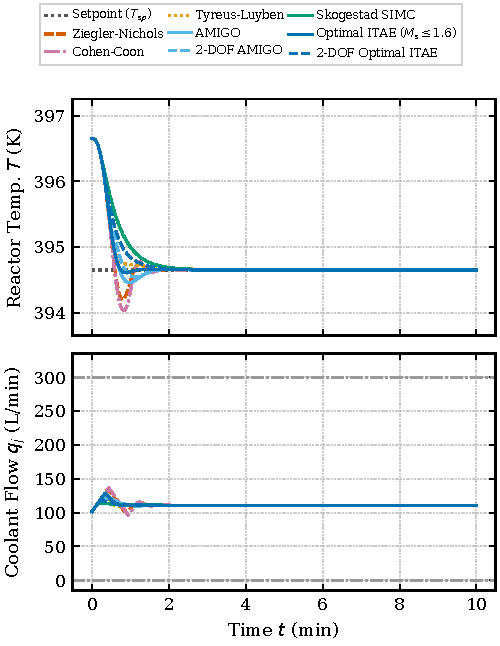
\includegraphics[width=\columnwidth]{figures/fig1_classical_benchmark.pdf}
    \caption{Nominal $-2$~K setpoint step (noise-free): reactor temperature and coolant flow for the eight PID tunings under the valve limits $[0, 300]$~L/min and $80$~L/min$^2$.}
    \label{fig:classical_benchmark}
\end{figure}

\begin{table*}[t]
\centering
\footnotesize
\caption{Nominal servo benchmark ($-2$~K setpoint step, noise-free) on the non-linear CSTR. FOPTD: $K=-0.1852$~K/(L/min), $\tau=0.6427$~min, $\theta=0.0935$~min. $M_s$ is evaluated on the dead-time FOPTD loop; TV includes the initial valve move from $\bar q_j$.}
\label{tab:classical_benchmark}
\resizebox{\ifdim\width>\textwidth\textwidth\else\width\fi}{!}{%
\begin{tabular}{lcccccccccc}
\toprule
Method & \(K_p\) & \(T_i\text{ (min)}\) & \(T_d\text{ (min)}\) & \(\beta\) & IAE & ITAE & TV (L/min) & \(M_p\text{ (\%)}\) & \(t_s\text{ (min)}\) & \(M_s\) \\
\midrule
Ziegler-Nichols & -44.56 & 0.187 & 0.047 & 1.0 & 0.940 & 0.316 & 81.9 & 22.6 & 1.38 & 4.14 \\
Cohen-Coon & -50.86 & 0.217 & 0.033 & 1.0 & 1.017 & 0.388 & 104.0 & 31.0 & 1.40 & 4.54 \\
Tyreus-Luyben & -28.10 & 0.779 & 0.056 & 1.0 & 0.917 & 0.336 & 48.8 & 0.0 & 1.64 & 2.32 \\
AMIGO & -17.79 & 0.327 & 0.045 & 1.0 & 0.925 & 0.308 & 40.4 & 9.7 & 1.44 & 1.45 \\
2-DOF AMIGO & -17.79 & 0.327 & 0.045 & 0.5 & 0.962 & 0.312 & 29.3 & 5.3 & 1.48 & 1.45 \\
Skogestad SIMC & -7.03 & 0.643 & 0.031 & 1.0 & 1.288 & 0.629 & 15.7 & 0.0 & 1.96 & 1.13 \\
Optimal ITAE ($M_s \leq 1.6$) & -23.55 & 0.465 & 0.032 & 1.0 & 0.827 & 0.204 & 48.6 & 2.2 & 0.94 & 1.60 \\
2-DOF Optimal ITAE & -23.55 & 0.465 & 0.032 & 0.5 & 1.084 & 0.424 & 25.0 & 0.0 & 1.62 & 1.60 \\
\bottomrule
\end{tabular}%
}
\end{table*}


With the directional rule of Eq.~\eqref{eq:clamping_antiwindup}, every tuning tracks the step. ZN and CC reach competitive errors ($\mathrm{IAE} = 0.940$ and $1.017$~K$\cdot$min) but with $M_s = 4.14$ and $4.54$, overshoots of $22.6\%$ and $31.0\%$ and $81.9$ and $104.0$~L/min of valve travel. Tyreus--Luyben gives $\mathrm{IAE} = 0.917$~K$\cdot$min without overshoot despite $M_s = 2.32$, and AMIGO ($M_s = 1.45$) gives $0.925$~K$\cdot$min with $9.7\%$ overshoot. Setpoint weighting reduces the AMIGO overshoot to $5.3\%$ and its travel from $40.4$ to $29.3$~L/min for a small increase in error ($0.962$~K$\cdot$min). SIMC ($M_s = 1.13$) is the most conservative tuning ($\mathrm{IAE} = 1.288$~K$\cdot$min, $\mathrm{TV} = 15.7$~L/min). Optimal ITAE, with its robustness constraint active ($M_s = 1.60$), is the fastest loop ($\mathrm{IAE} = 0.827$~K$\cdot$min, $\mathrm{ITAE} = 0.204$~K$\cdot$min$^2$, settling in $0.94$~min with $2.2\%$ overshoot); its 2-DOF variant removes the overshoot and roughly halves the travel ($25.0$~L/min) at $\mathrm{IAE} = 1.084$~K$\cdot$min.

\subsection{Anti-windup ablation}
\label{subsec:ablation}
Table~\ref{tab:antiwindup_ablation} repeats the nominal step with the same gains and valve but with the textbook amplitude-only, sign-blind clamping rule.

\begin{table*}[t]
\centering
\footnotesize
\caption{Anti-windup ablation on the nominal $-2$~K step (same gains, valve and protocol as Table~\ref{tab:classical_benchmark}): amplitude-only, sign-blind clamping (naive) versus the directional amplitude- and rate-aware rule of Eq.~\eqref{eq:clamping_antiwindup}.}
\label{tab:antiwindup_ablation}
\resizebox{\ifdim\width>\textwidth\textwidth\else\width\fi}{!}{%
\begin{tabular}{lcccccc}
\toprule
Method & IAE (naive) & \(M_p\) naive (\%) & TV naive (L/min) & IAE (directional) & \(M_p\) directional (\%) & TV directional (L/min) \\
\midrule
Ziegler-Nichols & 104.123 & 842.5 & 491.9 & 0.940 & 22.6 & 81.9 \\
Cohen-Coon & 102.668 & 842.5 & 478.4 & 1.017 & 31.0 & 104.0 \\
Tyreus-Luyben & 1.263 & 38.6 & 82.0 & 0.917 & 0.0 & 48.8 \\
AMIGO & 1.604 & 68.6 & 107.6 & 0.925 & 9.7 & 40.4 \\
Skogestad SIMC & 1.089 & 2.1 & 22.5 & 1.288 & 0.0 & 15.7 \\
Optimal ITAE ($M_s \leq 1.6$) & 1.508 & 66.0 & 112.2 & 0.827 & 2.2 & 48.6 \\
\bottomrule
\end{tabular}%
}
\end{table*}


The implementation changes the verdict on the empirical rules. With naive clamping, ZN and CC wind the integrator up while the valve is rate-limited: the temperature leaves the operating window, the overshoot reaches $842.5\%$ for both rules, and the IAE rises from $0.940$ to $104.123$~K$\cdot$min (ZN) and from $1.017$ to $102.668$~K$\cdot$min (CC). The same mechanism degrades the high-gain modern tunings, less dramatically: AMIGO overshoots by $68.6\%$ instead of $9.7\%$ and Optimal ITAE by $66.0\%$ instead of $2.2\%$, with two to three times the valve travel. The effect is not monotonic in the controller gain: for the low-gain SIMC loop the extra integration during the ramp shortens the transient ($\mathrm{IAE} = 1.089$ with naive against $1.288$~K$\cdot$min with directional clamping) at the cost of a small overshoot ($2.1\%$). The directional rule is therefore not uniformly faster; it is the rule that prevents loss of control of the high-gain loops. Published failures of the empirical rules on rate-limited exothermic loops should be read with the anti-windup implementation in mind.

\subsection{Design-model versus plant robustness}
\label{subsec:margins}
Figure~\ref{fig:sensitivity_magnitude} shows $|S(j\omega)|$ on the FOPTD, and Table~\ref{tab:loop_margins} compares $M_s$ and the phase margin on the FOPTD and on the exact linearization of the plant with the half-sample hold delay $\Delta t/2$.

\begin{figure}[t]
    \centering
    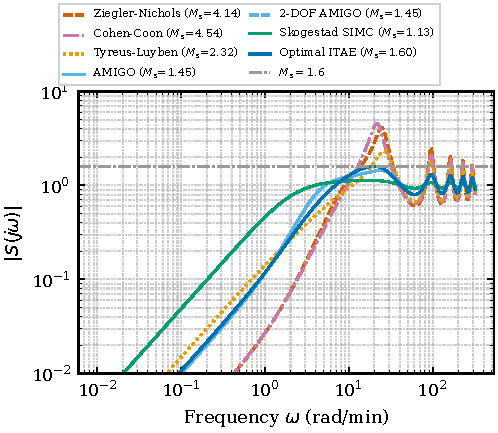
\includegraphics[width=0.92\columnwidth]{figures/fig_sensitivity_magnitude.pdf}
    \caption{Sensitivity magnitude $|S(j\omega)|$ on the identified dead-time FOPTD model. The 2-DOF variants share the loop of their 1-DOF counterparts.}
    \label{fig:sensitivity_magnitude}
\end{figure}

\begin{table*}[t]
\centering
\footnotesize
\caption{Sensitivity peak and phase margin of each PID loop on the identified FOPTD design model and on the exact Jacobian linearization of the CSTR at $\mathbf{x}_{ss}$ with the half-sample zero-order-hold delay $\Delta t/2 = 0.01$~min. Valve saturation and slew-rate limits are not part of either linear loop.}
\label{tab:loop_margins}
\resizebox{\ifdim\width>\textwidth\textwidth\else\width\fi}{!}{%
\begin{tabular}{lcccc}
\toprule
Method & \(M_s\) (FOPTD) & PM (FOPTD, \(^\circ\)) & \(M_s\) (lin.) & PM (lin., \(^\circ\)) \\
\midrule
Ziegler-Nichols & 4.14 & 36.6 & 1.57 & 38.4 \\
Cohen-Coon & 4.54 & 25.3 & 1.75 & 35.1 \\
Tyreus-Luyben & 2.32 & 72.3 & 1.15 & 71.1 \\
AMIGO & 1.45 & 59.3 & 1.26 & 53.9 \\
Skogestad SIMC & 1.13 & 81.7 & 1.11 & 78.7 \\
Optimal ITAE ($M_s \leq 1.6$) & 1.60 & 61.1 & 1.31 & 57.1 \\
\bottomrule
\end{tabular}%
}
\end{table*}


The sensitivity peak on the linearized plant is lower than on the FOPTD for every tuning, and strongly so for the high-gain rules (ZN: $4.14 \rightarrow 1.57$, CC: $4.54 \rightarrow 1.75$, TL: $2.32 \rightarrow 1.15$). Their peaks lie at high frequency, where the FOPTD delay keeps adding phase lag that the relative-degree-two plant of Eq.~\eqref{eq:g_true_exact} does not have; together with the rate limit, which clips the initial proportional kick into a bounded ramp, this explains why ZN and CC do not oscillate on the noise-free step. The phase margin, set near crossover, behaves differently: for the moderate-bandwidth designs the FOPTD is slightly optimistic (AMIGO: $59.3^\circ$ versus $53.9^\circ$, Optimal ITAE: $61.1^\circ$ versus $57.1^\circ$, SIMC: $81.7^\circ$ versus $78.7^\circ$), whereas for ZN and CC it is pessimistic ($36.6^\circ$ versus $38.4^\circ$ and $25.3^\circ$ versus $35.1^\circ$). The $M_s \le 1.6$ constraint imposed on the FOPTD is thus a conservative proxy for the peak sensitivity of the real loop, but the designer should allow for a loss of up to $5.4^\circ$ of phase margin at crossover. Neither linear loop contains the rate limit, which adds an amplitude-dependent phase lag during large moves; the table describes small-signal behaviour.

\subsection{Unmeasured load disturbances}
\label{subsec:load_results}
A feed temperature step $\Delta T_f = +5$~K at $t = 2$~min and a feed concentration step $\Delta C_{Af} = +0.2$~mol/L ($+20\%$) at $t = 8$~min were applied at constant setpoint with thermocouple noise $\sigma = 0.05$~K (Fig.~\ref{fig:disturbance_rejection}, Table~\ref{tab:load_disturbance}).

\begin{figure}[t]
    \centering
    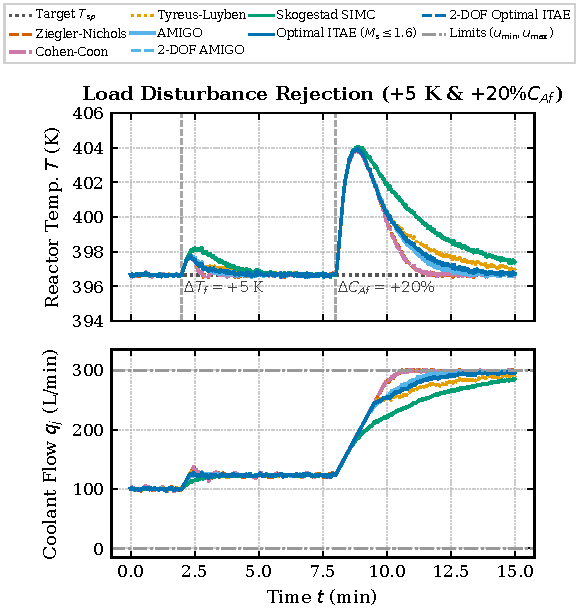
\includegraphics[width=\columnwidth]{figures/fig2_disturbance_rejection.pdf}
    \caption{Rejection of a $+5$~K feed temperature step at $t = 2$~min and a $+20\%$ feed concentration step at $t = 8$~min (sensor noise $\sigma = 0.05$~K).}
    \label{fig:disturbance_rejection}
\end{figure}

\begin{table*}[t]
\centering
\footnotesize
\caption{Regulatory performance under combined feed temperature ($+5$~K) and concentration ($+20\%$) load disturbances. $T(t_f) - T_{sp}$ is the true temperature error at $t_f = 15$~min.}
\label{tab:load_disturbance}
\resizebox{\ifdim\width>\textwidth\textwidth\else\width\fi}{!}{%
\begin{tabular}{lcccccc}
\toprule
Method & IAE & ITAE & TV (L/min) & Peak Dev (K) & Max Valve (L/min) & \(T(t_f) - T_{sp}\) (K) \\
\midrule
Ziegler-Nichols & 12.96 & 115.22 & 1097.8 & 7.26 & 300.0 & -0.01 \\
Cohen-Coon & 12.88 & 114.53 & 1108.8 & 7.22 & 300.0 & -0.01 \\
Tyreus-Luyben & 18.59 & 177.06 & 1091.7 & 7.32 & 293.6 & +0.35 \\
AMIGO & 15.27 & 139.03 & 1013.8 & 7.29 & 299.5 & +0.02 \\
2-DOF AMIGO & 15.27 & 139.03 & 1013.8 & 7.29 & 299.5 & +0.02 \\
Skogestad SIMC & 25.58 & 248.65 & 732.0 & 7.41 & 285.0 & +0.74 \\
Optimal ITAE ($M_s \leq 1.6$) & 16.20 & 150.00 & 1036.5 & 7.28 & 298.8 & +0.07 \\
2-DOF Optimal ITAE & 16.20 & 150.00 & 1036.5 & 7.28 & 298.8 & +0.07 \\
\bottomrule
\end{tabular}%
}
\end{table*}


All loops contain the excursion to $7.22$--$7.41$~K and return to the setpoint by integral action; at $t_f = 15$~min the remaining error ranges from $-0.01$~K (ZN, CC) to $+0.74$~K for SIMC, which is still settling. In regulation the ranking broadly follows the integral gain $K_p/T_i$ and reverses the servo ranking of the conservative designs: CC ($12.88$~K$\cdot$min), ZN ($12.96$), AMIGO ($15.27$) and Optimal ITAE ($16.20$) give the lowest error at $1013.8$--$1108.8$~L/min of valve travel, whereas SIMC is the slowest regulator ($25.58$~K$\cdot$min) with the lowest travel ($732.0$~L/min). The concentration step drives every loop to within $15$~L/min of the upper stop ($285.0$--$300.0$~L/min), i.e. close to the heat-removal limit of Section~\ref{sec:model}. The 2-DOF variants reproduce their 1-DOF metrics exactly (e.g. AMIGO and 2-DOF AMIGO: $15.27$~K$\cdot$min, $1013.8$~L/min), which confirms that setpoint weighting does not alter the disturbance response.

\subsection{Tracking error versus valve travel}
\label{subsec:pareto_results}
The trade-off between tracking accuracy and actuator wear was mapped by sweeping the SIMC closed-loop time constant over $\tau_c \in [0.015, 2.5]$~min ($45$ logarithmically spaced points) and by minimizing $\lambda\,\mathrm{IAE}/\mathrm{IAE}_0 + (1 - \lambda)\,\mathrm{TV}/\mathrm{TV}_0$ for $\lambda \in [0.05, 0.95]$ (Fig.~\ref{fig:pareto_iae_tv}, Table~\ref{tab:pareto_tradeoff}).

\begin{figure*}[t]
    \centering
    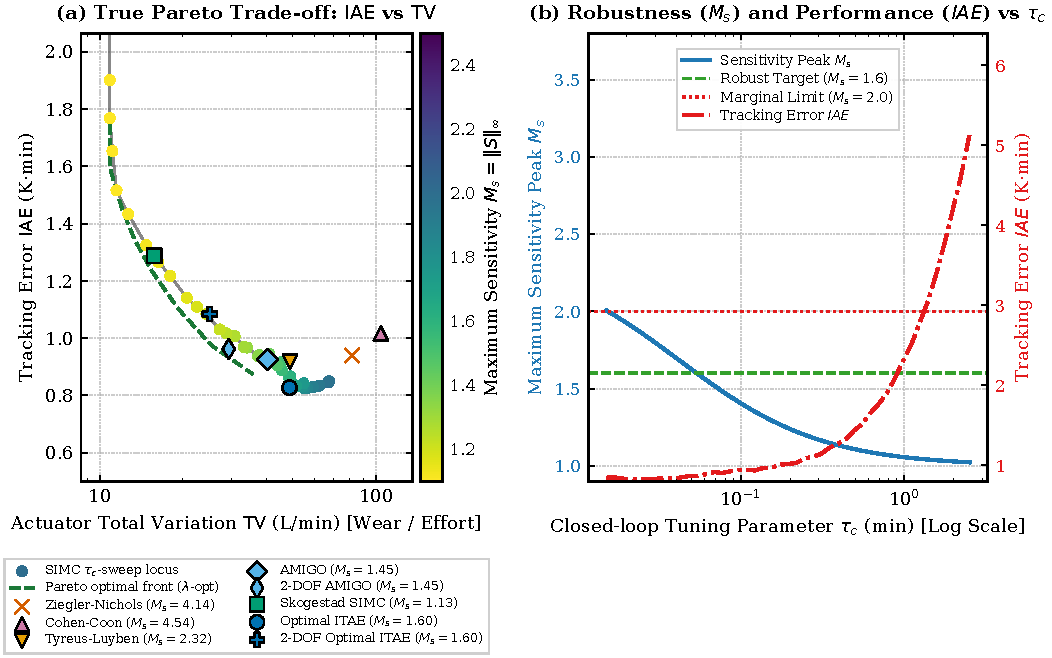
\includegraphics[width=0.92\textwidth]{figures/fig4_pareto_iae_tv.pdf}
    \caption{(a) SIMC $\tau_c$-sweep locus (colour: $M_s$), scalarized optimal front ($\lambda$-opt) and the discrete tunings in the $(\mathrm{TV}, \mathrm{IAE})$ plane (logarithmic TV axis); (b) $M_s$ and IAE as functions of $\tau_c$.}
    \label{fig:pareto_iae_tv}
\end{figure*}

\begin{table*}[t]
\centering
\footnotesize
\caption{Quantitative trade-off along the continuous Pareto frontier: impact of closed-loop tuning parameter $\tau_c$ and classical rules on robustness ($M_s$) and actuator effort ($TV$).}
\label{tab:pareto_tradeoff}
\resizebox{\ifdim\width>\textwidth\textwidth\else\width\fi}{!}{%
\begin{tabular}{lccccccc}
\toprule
Strategy & $K_{p}$ & $T_{i}$ (min) & $T_{d}$ (min) & $M_{s}$ & IAE (K$\cdot$min) & TV (L/min) & $M_{p}$ (\%) \\
\midrule
SIMC ($\tau_c=0.03$) & -28.08 & 0.49 & 0.03 & 1.79 & 0.83 & 54.2 & 0.3 \\
SIMC ($\tau_c=0.10$) & -18.28 & 0.64 & 0.03 & 1.41 & 0.95 & 41.0 & 0.0 \\
SIMC ($\tau_c=0.24$) & -10.27 & 0.64 & 0.03 & 1.20 & 1.08 & 24.3 & 0.0 \\
SIMC ($\tau_c=0.39$) & -7.19 & 0.64 & 0.03 & 1.13 & 1.27 & 16.3 & 0.0 \\
SIMC ($\tau_c=0.78$) & -3.97 & 0.64 & 0.03 & 1.07 & 1.90 & 10.9 & 0.0 \\
SIMC ($\tau_c=1.57$) & -2.09 & 0.64 & 0.03 & 1.04 & 3.40 & 10.9 & 0.0 \\
Ziegler-Nichols & -44.56 & 0.19 & 0.05 & 4.14 & 0.94 & 81.9 & 22.6 \\
Cohen-Coon & -50.86 & 0.22 & 0.03 & 4.54 & 1.02 & 104.0 & 31.0 \\
Tyreus-Luyben & -28.10 & 0.78 & 0.06 & 2.32 & 0.92 & 48.8 & 0.0 \\
AMIGO & -17.79 & 0.33 & 0.04 & 1.45 & 0.93 & 40.4 & 9.7 \\
2-DOF AMIGO & -17.79 & 0.33 & 0.04 & 1.45 & 0.96 & 29.3 & 5.3 \\
Skogestad SIMC & -7.03 & 0.64 & 0.03 & 1.13 & 1.29 & 15.7 & 0.0 \\
Optimal ITAE ($M_s \leq 1.6$) & -23.55 & 0.47 & 0.03 & 1.60 & 0.83 & 48.6 & 2.2 \\
2-DOF Optimal ITAE & -23.55 & 0.47 & 0.03 & 1.60 & 1.08 & 25.0 & 0.0 \\
\bottomrule
\end{tabular}%
}
\end{table*}


Along the SIMC locus the error decreases monotonically as $\tau_c$ shrinks ($1.90$, $1.27$, $1.08$, $0.95$ and $0.83$~K$\cdot$min for $\tau_c = 0.78$, $0.39$, $0.24$, $0.10$ and $0.03$~min) while $M_s$ rises from $1.07$ to $1.79$ and the travel from $10.9$ to $54.2$~L/min: speed is bought with robustness, and with a correct anti-windup the rate limit creates no interior optimum. For $\tau_c \ge 0.78$~min the travel reaches its floor of $10.9$~L/min, the net change of steady-state coolant flow required by the new setpoint. The scalarized front lies slightly below the SIMC locus, so a free PID improves on SIMC by a small margin at equal travel. SIMC, 2-DOF AMIGO and 2-DOF Optimal ITAE lie close to the front; AMIGO, TL and Optimal ITAE sit on its high-gain branch; ZN and CC are dominated, with more error and more travel than Optimal ITAE at $2.6$ to $2.8$ times its design $M_s$.

\subsection{Robustness to sensor noise}
\label{subsec:noise_results}
Gaussian thermocouple noise $\sigma \in \{0.0, 0.1, 0.2, 0.5, 1.0\}$~K was applied to the nominal step with $30$ independent realizations per level and tuning, i.e. $1200$ closed-loop runs (Fig.~\ref{fig:noise_sensitivity}, Table~\ref{tab:noise_sensitivity}).

\begin{figure}[t]
    \centering
    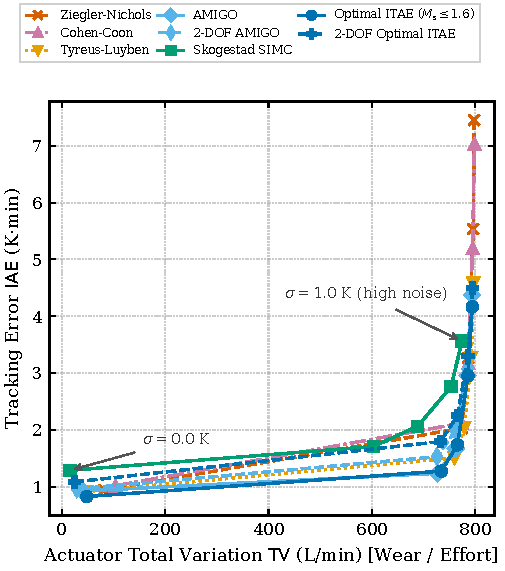
\includegraphics[width=0.92\columnwidth]{figures/fig_noise_sensitivity.pdf}
    \caption{Mean true-temperature IAE versus mean valve travel as the sensor noise grows from $\sigma = 0$ to $1.0$~K ($30$ runs per point).}
    \label{fig:noise_sensitivity}
\end{figure}

\begin{table*}[t]
\centering
\footnotesize
\caption{Sensitivity of tracking error (IAE) and actuator effort (TV) to measurement noise levels across $30$ Monte Carlo runs.}
\label{tab:noise_sensitivity}
\resizebox{\ifdim\width>\textwidth\textwidth\else\width\fi}{!}{%
\begin{tabular}{lccc}
\toprule
Method & Noise $\sigma$ (K) & IAE (mean $\pm$ std) & TV (L/min) \\
\midrule
Ziegler-Nichols & 0.0 & 0.94 $\pm$ 0.00 & 81.9 $\pm$ 0.0 \\
Ziegler-Nichols & 0.1 & 2.03 $\pm$ 0.18 & 773.7 $\pm$ 4.6 \\
Ziegler-Nichols & 0.2 & 3.26 $\pm$ 0.45 & 786.3 $\pm$ 3.9 \\
Ziegler-Nichols & 0.5 & 5.54 $\pm$ 1.26 & 796.0 $\pm$ 2.1 \\
Ziegler-Nichols & 1.0 & 7.45 $\pm$ 1.90 & 798.0 $\pm$ 1.9 \\
Cohen-Coon & 0.0 & 1.02 $\pm$ 0.00 & 104.0 $\pm$ 0.0 \\
Cohen-Coon & 0.1 & 2.12 $\pm$ 0.15 & 773.1 $\pm$ 4.4 \\
Cohen-Coon & 0.2 & 3.16 $\pm$ 0.40 & 786.2 $\pm$ 4.7 \\
Cohen-Coon & 0.5 & 5.19 $\pm$ 1.11 & 794.7 $\pm$ 2.8 \\
Cohen-Coon & 1.0 & 7.03 $\pm$ 1.60 & 798.3 $\pm$ 1.6 \\
Tyreus-Luyben & 0.0 & 0.92 $\pm$ 0.00 & 48.8 $\pm$ 0.0 \\
Tyreus-Luyben & 0.1 & 1.51 $\pm$ 0.07 & 759.4 $\pm$ 7.5 \\
Tyreus-Luyben & 0.2 & 2.04 $\pm$ 0.18 & 778.8 $\pm$ 4.3 \\
Tyreus-Luyben & 0.5 & 3.27 $\pm$ 0.59 & 792.4 $\pm$ 3.0 \\
Tyreus-Luyben & 1.0 & 4.58 $\pm$ 0.81 & 796.1 $\pm$ 2.3 \\
AMIGO & 0.0 & 0.93 $\pm$ 0.00 & 40.4 $\pm$ 0.0 \\
AMIGO & 0.1 & 1.24 $\pm$ 0.05 & 727.0 $\pm$ 7.7 \\
AMIGO & 0.2 & 1.67 $\pm$ 0.14 & 762.2 $\pm$ 6.5 \\
AMIGO & 0.5 & 2.96 $\pm$ 0.46 & 785.0 $\pm$ 5.0 \\
AMIGO & 1.0 & 4.38 $\pm$ 0.92 & 793.5 $\pm$ 1.9 \\
2-DOF AMIGO & 0.0 & 0.96 $\pm$ 0.00 & 29.3 $\pm$ 0.0 \\
2-DOF AMIGO & 0.1 & 1.53 $\pm$ 0.07 & 725.8 $\pm$ 7.3 \\
2-DOF AMIGO & 0.2 & 1.99 $\pm$ 0.13 & 761.7 $\pm$ 5.7 \\
2-DOF AMIGO & 0.5 & 3.07 $\pm$ 0.41 & 785.7 $\pm$ 4.3 \\
2-DOF AMIGO & 1.0 & 4.46 $\pm$ 0.72 & 793.3 $\pm$ 2.9 \\
Skogestad SIMC & 0.0 & 1.29 $\pm$ 0.00 & 15.7 $\pm$ 0.0 \\
Skogestad SIMC & 0.1 & 1.71 $\pm$ 0.07 & 603.0 $\pm$ 11.4 \\
Skogestad SIMC & 0.2 & 2.06 $\pm$ 0.11 & 688.5 $\pm$ 8.8 \\
Skogestad SIMC & 0.5 & 2.76 $\pm$ 0.20 & 753.1 $\pm$ 5.3 \\
Skogestad SIMC & 1.0 & 3.56 $\pm$ 0.34 & 774.2 $\pm$ 4.6 \\
Optimal ITAE ($M_s \leq 1.6$) & 0.0 & 0.83 $\pm$ 0.00 & 48.6 $\pm$ 0.0 \\
Optimal ITAE ($M_s \leq 1.6$) & 0.1 & 1.27 $\pm$ 0.05 & 734.1 $\pm$ 6.8 \\
Optimal ITAE ($M_s \leq 1.6$) & 0.2 & 1.74 $\pm$ 0.12 & 765.5 $\pm$ 6.4 \\
Optimal ITAE ($M_s \leq 1.6$) & 0.5 & 2.95 $\pm$ 0.48 & 785.7 $\pm$ 3.0 \\
Optimal ITAE ($M_s \leq 1.6$) & 1.0 & 4.16 $\pm$ 0.63 & 794.0 $\pm$ 3.3 \\
2-DOF Optimal ITAE & 0.0 & 1.08 $\pm$ 0.00 & 25.0 $\pm$ 0.0 \\
2-DOF Optimal ITAE & 0.1 & 1.80 $\pm$ 0.07 & 732.5 $\pm$ 6.7 \\
2-DOF Optimal ITAE & 0.2 & 2.25 $\pm$ 0.13 & 765.4 $\pm$ 5.5 \\
2-DOF Optimal ITAE & 0.5 & 3.30 $\pm$ 0.38 & 785.9 $\pm$ 3.5 \\
2-DOF Optimal ITAE & 1.0 & 4.50 $\pm$ 0.63 & 794.5 $\pm$ 2.3 \\
\bottomrule
\end{tabular}%
}
\end{table*}


Since the IAE is evaluated on the true temperature, the table measures how much sensor noise each loop converts into real thermal deviation. Valve travel saturates first: $\mathrm{TV}$ is bounded by $|u_0 - \bar q_j| + S_{\max}t_f \approx 800$~L/min, and all tunings approach this ceiling at $\sigma = 0.1$--$0.2$~K (ZN: $773.7$, Optimal ITAE: $734.1$~L/min at $0.1$~K), SIMC being the least affected ($15.7 \rightarrow 603.0$~L/min). Under heavy noise the nominal ranking reverses. At $\sigma = 1.0$~K SIMC gives the lowest true-temperature error ($3.56 \pm 0.34$~K$\cdot$min), followed by Optimal ITAE ($4.16 \pm 0.63$), AMIGO ($4.38 \pm 0.92$) and TL ($4.58 \pm 0.81$), while the empirical rules give the largest (CC: $7.03 \pm 1.60$, ZN: $7.45 \pm 1.90$~K$\cdot$min). This is where the small margins of ZN and CC become decisive: noise excites the high-frequency band where their sensitivity peaks lie (Fig.~\ref{fig:sensitivity_magnitude}). The derivative filter bounds the high-frequency controller gain at $|K_p|(1 + N)$, but with $|K_p|$ between $7.03$ and $50.86$ this still maps $0.1$~K of noise into several L/min per sample; a measurement filter or a lower $N$ is needed where valve wear matters.

\subsection{Global sensitivity under simultaneous uncertainty}
\label{subsec:sobol_results}
Sobol' indices \cite{sobol2001global, saltelli2010variance} decompose the variance of a closed-loop metric $Y \in \{\mathrm{IAE}, \mathrm{TV}\}$ over uncertain factors $\boldsymbol{\xi}$:
\begin{equation}
    S_i = \frac{\mathbb{V}_{\xi_i}\!\left[\mathbb{E}(Y \mid \xi_i)\right]}{\mathbb{V}(Y)}, \qquad S_{Ti} = \frac{\mathbb{E}_{\boldsymbol{\xi}_{\sim i}}\!\left[\mathbb{V}(Y \mid \boldsymbol{\xi}_{\sim i})\right]}{\mathbb{V}(Y)},
    \label{eq:sobol}
\end{equation}
where $S_i$ is the share of variance explained by $\xi_i$ alone and $S_{Ti} \ge S_i$ adds its interactions. The factors were sampled uniformly on $E_a/R \in [0.97, 1.03]$, $UA \in [0.65, 1.05]$ (both relative to nominal), $C_{Af} \in [0.85, 1.15]$~mol/L and a pure sensor dead time $\theta_{\text{sensor}} \in [0, 0.1]$~min, for a $-2$~K step. Indices were estimated with Saltelli sampling and the SALib estimators \cite{herman2017salib} ($N = 512$, $3072$ runs per tuning) for five representative tunings (Fig.~\ref{fig:sobol}, Table~\ref{tab:sobol_sensitivity}); every table satisfies $S_{Ti} \ge S_i - 0.01$.

\begin{figure*}[t]
    \centering
    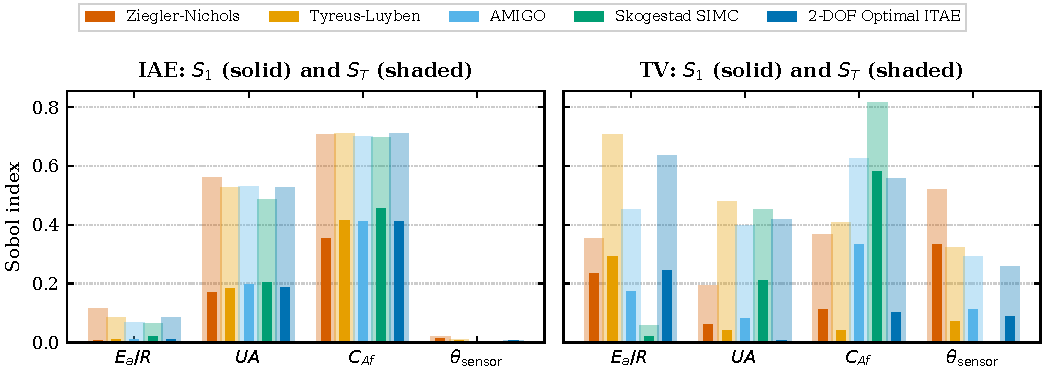
\includegraphics[width=0.92\textwidth]{figures/fig_sobol_indices.pdf}
    \caption{First-order ($S_1$, solid) and total-order ($S_T$, shaded) Sobol indices of IAE (left) and TV (right) for five PID tunings.}
    \label{fig:sobol}
\end{figure*}

\begin{table*}[t]
\centering
\footnotesize
\caption{Global Sobol indices (Saltelli sampling, $N=512$, $3072$ closed-loop runs per controller) of IAE and TV for a $-2$~K setpoint step under simultaneous uncertainty $E_a/R \in [0.97, 1.03]$, $UA \in [0.65, 1.05]\,UA_{\mathrm{nom}}$, $C_{Af} \in [0.85, 1.15]$~mol/L and sensor dead time $\theta_{\mathrm{sensor}} \in [0, 0.1]$~min.}
\label{tab:sobol_sensitivity}
\resizebox{\ifdim\width>\textwidth\textwidth\else\width\fi}{!}{%
\begin{tabular}{lccccc}
\toprule
Controller & Parameter & $S_1$ (IAE) & $S_T$ (IAE) & $S_1$ (TV) & $S_T$ (TV) \\
\midrule
Ziegler-Nichols & $E_a/R$ & 0.006 & 0.113 & 0.234 & 0.350 \\
Ziegler-Nichols & $UA$ & 0.168 & 0.559 & 0.060 & 0.193 \\
Ziegler-Nichols & $C_{Af}$ & 0.354 & 0.703 & 0.111 & 0.365 \\
Ziegler-Nichols & $\theta_{\mathrm{sensor}}$ & 0.013 & 0.017 & 0.331 & 0.519 \\
Tyreus-Luyben & $E_a/R$ & 0.009 & 0.083 & 0.292 & 0.705 \\
Tyreus-Luyben & $UA$ & 0.183 & 0.523 & 0.041 & 0.475 \\
Tyreus-Luyben & $C_{Af}$ & 0.414 & 0.708 & 0.041 & 0.404 \\
Tyreus-Luyben & $\theta_{\mathrm{sensor}}$ & 0.006 & 0.007 & 0.070 & 0.320 \\
AMIGO & $E_a/R$ & 0.008 & 0.067 & 0.174 & 0.451 \\
AMIGO & $UA$ & 0.198 & 0.527 & 0.081 & 0.396 \\
AMIGO & $C_{Af}$ & 0.410 & 0.696 & 0.334 & 0.623 \\
AMIGO & $\theta_{\mathrm{sensor}}$ & 0.003 & 0.001 & 0.111 & 0.291 \\
Skogestad SIMC & $E_a/R$ & 0.018 & 0.063 & 0.021 & 0.057 \\
Skogestad SIMC & $UA$ & 0.205 & 0.485 & 0.211 & 0.449 \\
Skogestad SIMC & $C_{Af}$ & 0.454 & 0.695 & 0.580 & 0.813 \\
Skogestad SIMC & $\theta_{\mathrm{sensor}}$ & 0.000 & 0.000 & 0.002 & 0.001 \\
2-DOF Optimal ITAE & $E_a/R$ & 0.008 & 0.083 & 0.246 & 0.634 \\
2-DOF Optimal ITAE & $UA$ & 0.186 & 0.525 & 0.007 & 0.415 \\
2-DOF Optimal ITAE & $C_{Af}$ & 0.409 & 0.707 & 0.100 & 0.554 \\
2-DOF Optimal ITAE & $\theta_{\mathrm{sensor}}$ & 0.005 & 0.005 & 0.087 & 0.257 \\
\bottomrule
\end{tabular}%
}
\end{table*}


The decomposition shows that robustness changes what drives the variance. For every tuning, the variance of IAE is explained by feed concentration ($S_T = 0.695$--$0.708$) and heat-transfer capacity ($S_T = 0.485$--$0.559$), i.e. by how much heat must be removed and how much can be removed; the activation energy ($S_T = 0.063$--$0.113$) and the sensor dead time ($S_T \le 0.017$) contribute little. Valve activity tells the tunings apart. For SIMC its variance follows the physical load ($C_{Af}$: $S_T = 0.813$) and is insensitive to the sensor delay ($S_T = 0.001$). For the low-margin loops kinetics and delay matter: the TV of ZN is dominated by $\theta_{\text{sensor}}$ ($S_1 = 0.331$, $S_T = 0.519$), and those of TL and 2-DOF Optimal ITAE by $E_a/R$ ($S_T = 0.705$ and $0.634$). For every tuning $S_T$ substantially exceeds $S_1$ (e.g. TL, $UA$, TV: $S_1 = 0.041$, $S_T = 0.475$): the uncertainties act jointly, largely through saturation, so one-at-a-time robustness tests underestimate the effect of combined deviations.

\subsection{Limitations}
The study uses one reactor model with constant physical properties and constant $UA$, a valve without deadband or stiction, and Gaussian white measurement noise. The margins of Table~\ref{tab:loop_margins} are small-signal results that ignore the rate limit. The tuning comparison is restricted to fixed-gain PID control; gain scheduling and model-based controllers are outside its scope.


\section{Conclusions}\label{sec:conclusion}
Eight PID tunings were compared on a three-state exothermic CSTR whose cooling valve is limited in amplitude and in slew rate, under a single protocol with true-temperature metrics. Four conclusions follow.
\begin{enumerate}
    \item \textbf{The anti-windup implementation can decide the verdict on a tuning rule.} With directional clamping that accounts for amplitude and rate saturation and for the sign of the reverse-acting loop, every tuning tracks the nominal step; with the textbook amplitude-only rule, ZN and CC lose temperature control ($\mathrm{IAE}$ of $104.123$ and $102.668$ instead of $0.940$ and $1.017$~K$\cdot$min) and the high-gain modern tunings overshoot several times more. Comparisons that report the failure of empirical rules should state their anti-windup logic.
    \item \textbf{Robustness, not stability, separates the tunings.} The small margins of ZN and CC ($M_s = 4.14$ and $4.54$ on the design model) are masked on a clean step by the relative-degree-two plant and the rate limit, but under sensor noise they produce the largest thermal deviation, about twice that of SIMC at $\sigma = 1$~K. The FOPTD design model is a conservative proxy for the peak sensitivity of the real loop but can overestimate the phase margin by up to $5.4^\circ$.
    \item \textbf{Constrained optimization and setpoint weighting give the best servo compromise.} Multi-start ITAE optimization with $M_s \le 1.6$ on the dead-time loop yields the fastest robust PID ($\mathrm{IAE} = 0.827$~K$\cdot$min, constraint active), while a single-start search stops at a PI-like local optimum. Setpoint weighting reduces overshoot and valve travel for AMIGO and Optimal ITAE without changing their disturbance response, and the SIMC locus shows that tracking speed is bought with robustness along a front without interior optimum.
    \item \textbf{Tracking-error variance is governed by physics.} Under simultaneous uncertainty the IAE variance of every tuning is explained mainly by feed concentration and heat-transfer capacity, i.e. by the heat-removal limit of the reactor, whereas the valve activity of low-margin loops is driven by kinetics and sensor dead time.
\end{enumerate}
The released code reproduces every table and figure and accepts new controllers behind the same interface, so that future tuning methods, and nonlinear or learning-based controllers, can be compared with these robust PID baselines under identical plant, actuator and protocol. Future work will extend the analysis to gain-scheduled PID and to operating points inside the open-loop unstable region.


\section*{Data and code availability}
The simulation code, controllers, campaign scripts and the CSV files behind every table and figure are available at \url{https://github.com/Marques-svnt/IC-PID-Neural-Agents}.

\section*{Declaration of competing interest}
The authors declare that they have no known competing financial interests or personal relationships that could have appeared to influence the work reported in this paper.

\section*{Acknowledgements}
This research was supported in part by the Brazilian National Council for Scientific and Technological Development (CNPq), the Bahia State Research Foundation (FAPESB), and PROIC-UESC under Grant 34/2026.

\bibliographystyle{elsarticle-num}
\bibliography{references}

\end{document}
